\section{Experimental Methods}\label{sec:methods}
% \begin{enumerate}
% \item \cmark  Experimental methods: (how we collect the %time series and what the times series areThis should be HPM %PAPI, which programs we model
%\item \cmark program descriptions and relevant citations
%\subitem \cmark description of \col
%\subitem \cmark description of \gcc
%\subitem \cmark description of \svd 
%\subitem \cmark description of svd regimes
% \end{enumerate}


% \subsection{Time Series Collection}

The time-series data for these experiments was collected on an Intel
Core\textsuperscript{\textregistered} i7-2600-based machine running
the 2.6.38-8 Linux kernel.  This particular microprocessor chip has
eight processing units, a clock rate of 3.40GHz, and a cache size of
8192 KB.  We gathered performance traces during the execution of three
different programs---the simple \col loop whose performance is
depicted in Figure~\ref{fig:col-ipc}, as well as two more-complex
programs: one from the SPEC 2006CPU benchmark suite (\gcc), and one
from the LAPACK linear algebra package (\svd).  In these experiments,
the scalar observation $x_{i}$ at time $i$ was a measurement of how
well each program was able to exploit the native parellelism of the i7
chip.  To record these measurements, we used the {\tt libpfm4}
library, via PAPI
% 
% \footnote{Performance Application Programming Interface}
% 
5.2~\cite{papi}, to stop program execution at 100,000-instruction
intervals and read the contents of the CPU's onboard hardware
performance monitors\footnote{These specialty registers are built into
  modern microprocessors for the purpose of on-board monitoring and
  storage of performance data.}, which we had programmed to count how
many instructions were executed in each clock cycle (IPC).  For an
in-depth description of this custom-measurement infrastructure,
including discussion of the implications of the sampling interval,
please see \cite{zach-IDA10,mytkowicz09,todd-phd}.  For statistical
validation, we collected 15 performance traces from each of the three
programs.  These traces, and the processes that generated them, are
described in more depth in the rest of this section.


% Obviously using a system to measure itself can cause
% interference--i.e, are you measuring the generating process cleanly or
% are you adding noise to the process?---but due diligence was put into
% monitoring the generating process of these time series without
% interfering with it in a significant way.


% \subsection{The Programs: [[Maybe The generating processes]]{\color{blue} EDITABLE}}
% We collect performance traces of processor efficiency (IPC) of three
% exemplar programs, [[If we change the title of the section, add this:
%     which act as our generating processes]]---a simple
% microkernel(\col) and two complex programs: one from the SPEC 2006CPU
% benchmark suite (\gcc), and one from LAPACK (\svd). In this section we
% provide a quick explanation of each program as well as an example
% performance trace (Seen in Figures
% \ref{fig:col-ts}-\ref{fig:svd-ts-colored}.

\col is a simple three-line C program that repeatedly initializes the
upper triangle of a 2048 $\times$ 2048 matrix in column-major order.
As mentioned in the previous section, this simple program exhibits
surprisingly complicated behavior~\cite{mytkowicz09}.  A time series
of the processor utilization during the execution this program is
shown in Figure~\ref{fig:col-ts}.
\begin{figure}[htbp]
  \centering
    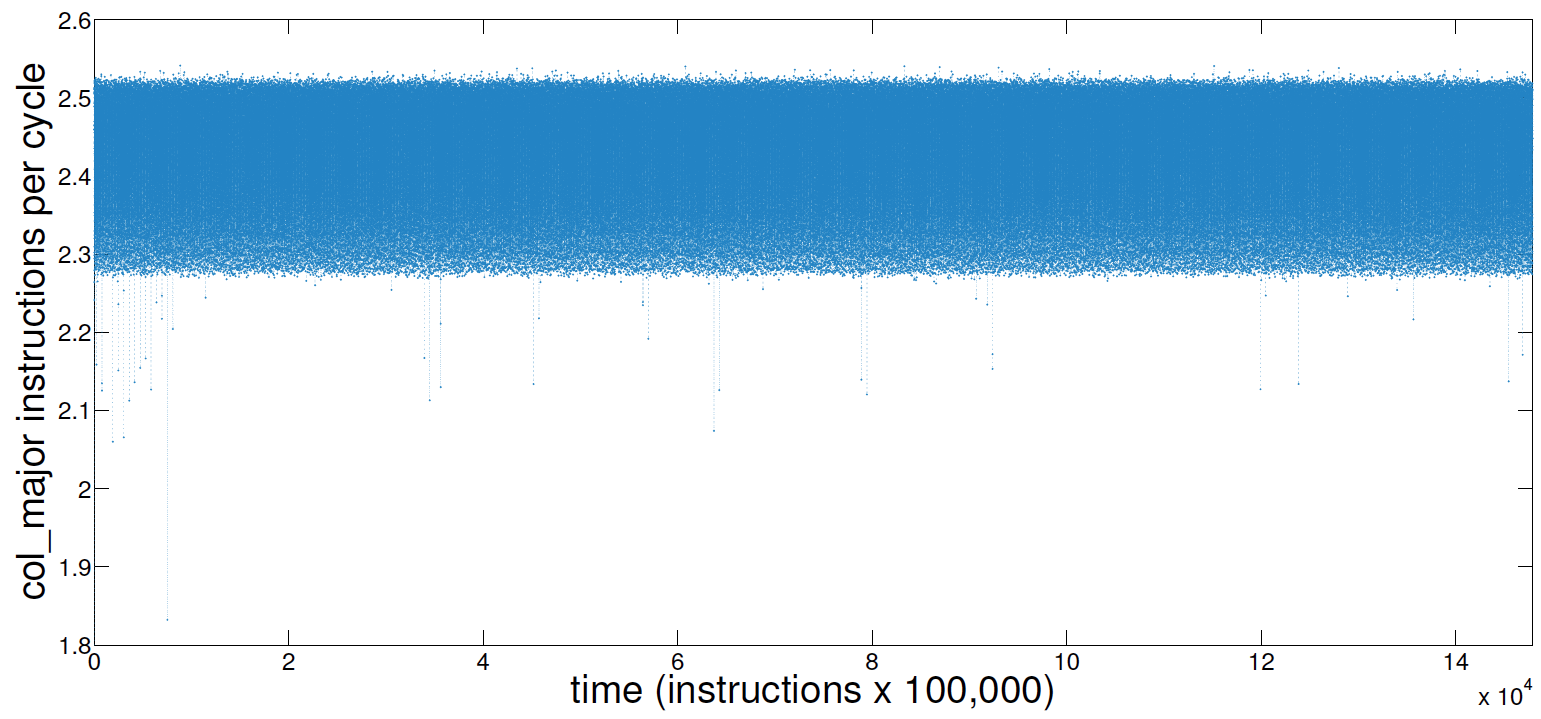
\includegraphics[width=\columnwidth]{figs/colFullTS}
    \caption{The instructions executed per CPU clock cycle (IPC)
      during the execution of \col.  Each point is the average IPC
      during a 100,000 instruction period. Figure~\ref{fig:col-ipc} is
      a closeup of the first part of this signal.  }
    \label{fig:col-ts}
  
  \end{figure}

The SPEC CPU2006 benchmark suite \cite{spec} is a collection of
complicated programs that are used in the computer science community
to assess and compare the performance of different computers.  \gcc is
a member of that suite.
% 
% This program is written by Richard Stallman and is based on Version
% 3.2 of {\tt gcc}. This benchmark essentially runs as a compiler with
% many of its optimization flags enabled, compiling a series of input
% files and generating x86-64 assembly code files intended for execution
% on AMD Opteron processors\cite{spec}. 
% 
It is a \emph{compiler}: a program that translates code written in the
C language into a lower-level format that can be executed by the
processor chip.  Its behavior is far more complicated than that of
\col, as is clear from Figure~\ref{fig:gcc-ts}.
  \begin{figure}[t]
  \centering
    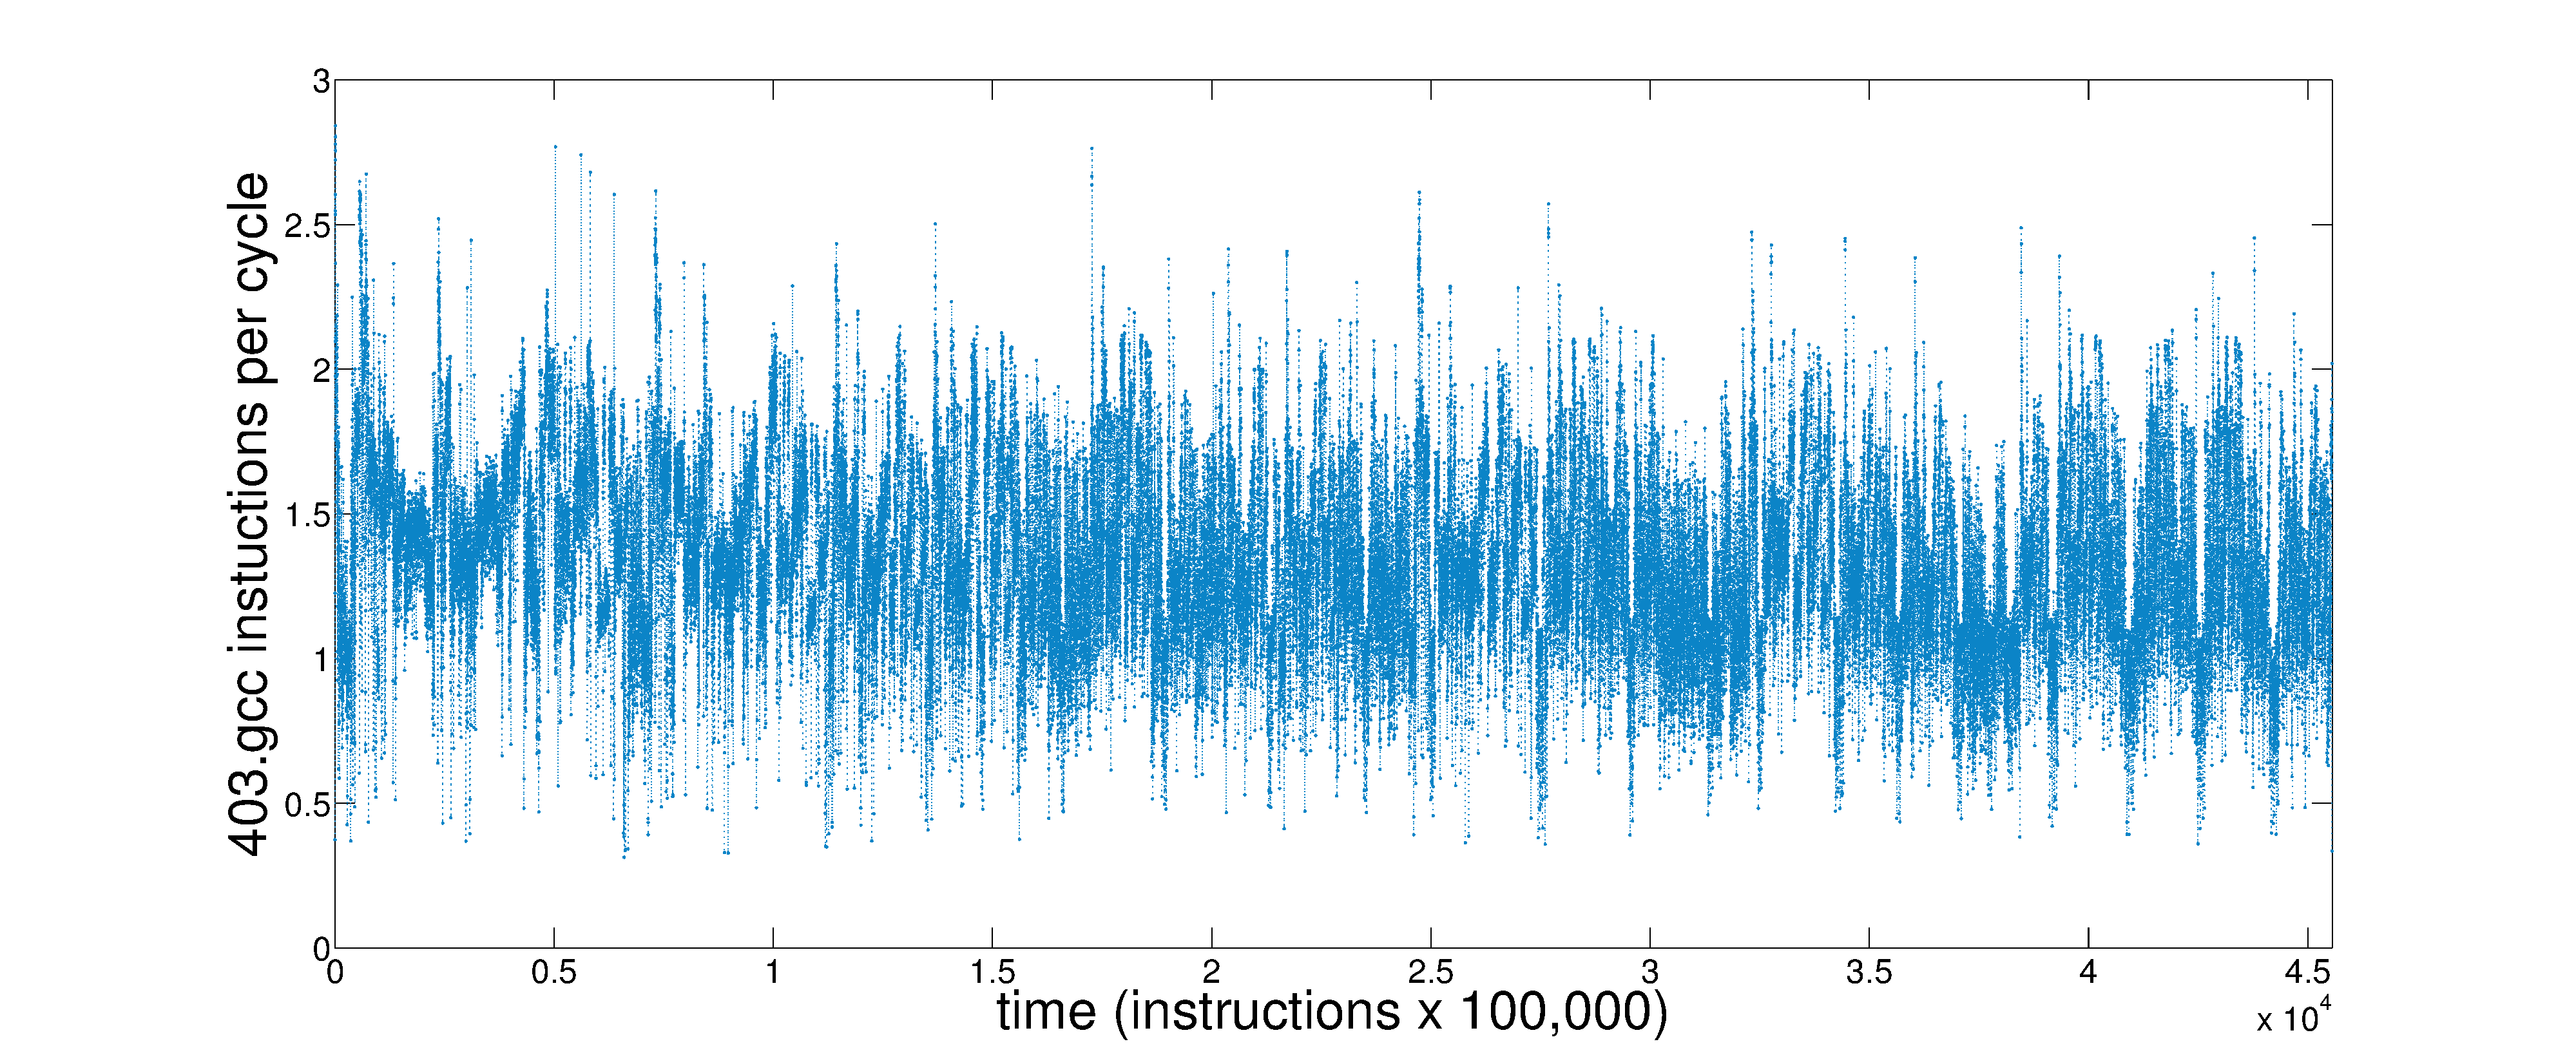
\includegraphics[width=\columnwidth]{figs/gccfullts}
    \caption{The instructions executed per CPU clock cycle (IPC)
      during the execution of \gcc. Each point is the average IPC
      during a 100,000 instruction period.}
    \label{fig:gcc-ts}
  \end{figure}
Unlike \col, where the processor utilization is quite structured,
\gcc's performance appears almost random.

\svd is a Fortran program from the LAPACK linear algebra package
\cite{lapack}.  It calculates the singular value decomposition of an
rectangular $M$ by $N$ real-valued matrix.  For our experiments, we
choose $M=750$ and $N=1000$ and generated the matrix entries randomly.
% 
% \footnote{Multiple randomly generated matrices were
%   investigated but no measurable effect was present in the resulting
%   time series.}. 
% 
The behavior of this program as it computes the singular values of
this matrix is very interesting, as shown in Figure
\ref{fig:svd-ts-colored}.  As the code moves though its different
phases---diagonalizing the matrix, computing its transpose,
multiplying, etc.---the processor utilization changes quite radically,
as shown in Figure~\ref{fig:svd-ts-colored}.
\begin{figure}[t]
    \centering
    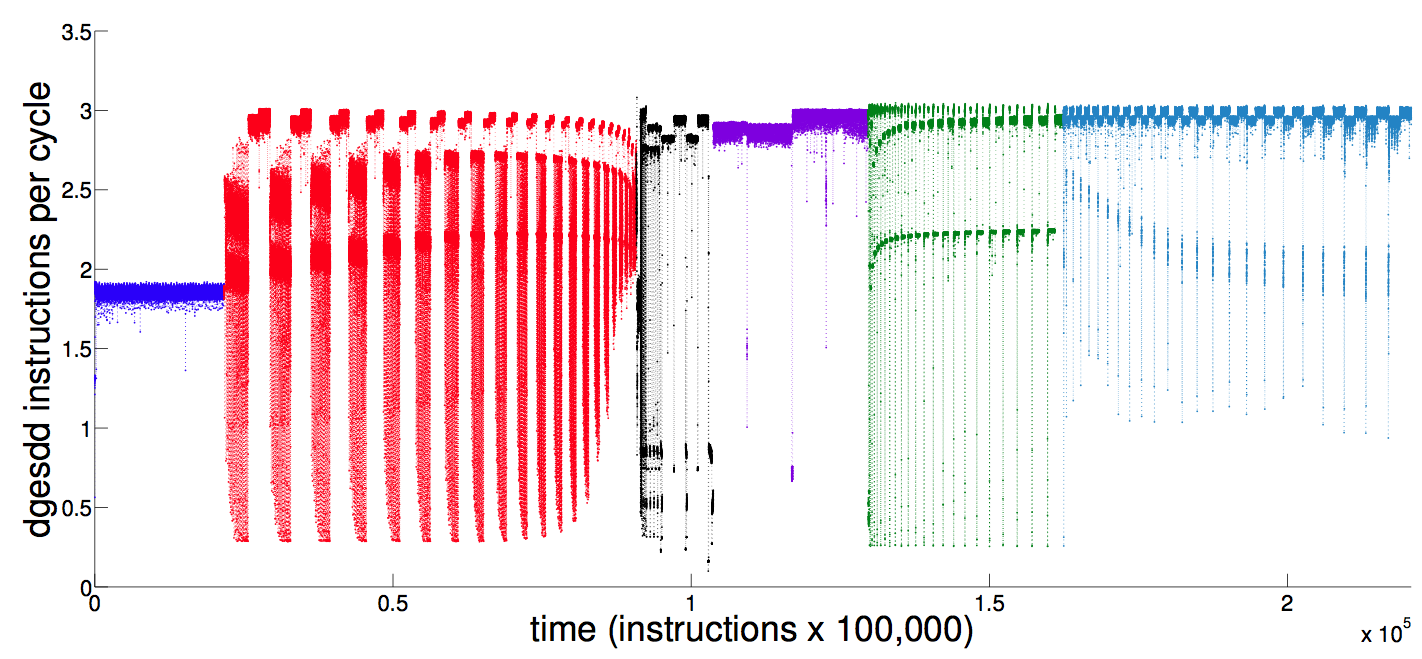
\includegraphics[width=\columnwidth]{figs/SVD1RegimesColored}
    \caption{The instructions executed per CPU clock cycle (IPC)
      during the execution of \svd. Each point is the average IPC
      during a 100,000 instruction period.  The colors refer to different
``regimes'' of the signal, as discussed in the text.}
    \label{fig:svd-ts-colored}
  \end{figure}
For the first $\sim$27,000 instructions{\color{red}[[Joshua,I am not sure about this, I think it is more instructions than that. 27,000 instructions are aggregated  in the first point of the time series (every 100,000 instructions is 1 point)...Liz how did you calculate this, I think it should be 21,000*100,000]]}, roughly 1.8 instructions are
executed per cycle, on the average, by the eight processing units on
this chip.  After that, the IPC moves through a number of different
oscillatory regimes, which we have color-coded in the figure in order
to make textual cross-references easy to track and understand.

This wide range of behaviors provides a unique advantage, for the
purposes of this paper, in that a number of different generating
processes---with a wide range of complexities---are at work at
different points in a single time series.  The complexity of \col and
\gcc in Figures~\ref{fig:col-ts} and \ref{fig:gcc-ts} appears to be
far more consistent over time---probably the result of a single
generating process.  \svd, in contrast, has multiple regimes, each the
result of a different generating process.  To take advantage of this,
we split the signal into six different segments, thereby obtaining an
array of examples for the analyses in the following sections.  For
notational convenience, we refer to these 90 time series\footnote{15
  runs, each with six regimes} as {\tt dgesdd$_i$} with $i \in
\{1\dots6\}$ where $i$ corresponds to one of the six color-coded
segments of \svd, ordered from left to right.  These segments, which
were determined visually, are shown in different colors in
Figure~\ref{fig:svd-ts-colored}.  Visual decomposition is subjective,
of course, particularly since the regimes exhibit some fractal
structure\footnote{It should be noted that a version of the complexity
  metric discussed in Section~\ref{sec:meaComplex} has been used to
  detect seizures in brainwave data \cite{cao2004det}, which can be
  viewed as regime detection.  The purpose of this paper is \emph{not}
  to rigorously explore regime detection but to explore quantifying
  complexity of a time series.}.  Thus, it may the case that more than
one generating process may be at work in each of our segments.  This
is a factor in the discussion of Section~\ref{sec:results}.

%[[Orphan citation?]] For regimes \cite{cao2004det}
